

\documentclass{beamer}

% --- THEME AND COLOR ---
\usetheme{Madrid}
\usecolortheme{default}

% --- PACKAGES ---
\usepackage{graphicx}
\usepackage{amsmath}
\usepackage{booktabs}   % For professional-looking tables (\toprule, etc.)
\usepackage{subcaption} % For subFigures
\usepackage{multirow}   % For multi-row cells in tables
\usepackage{siunitx}    % For better number and unit formatting
\usepackage{tikz}       % For drawing diagrams

% --- TIKZ LIBRARIES (Consolidated into one line) ---
\usetikzlibrary{shapes.geometric, arrows.meta, positioning, fit, calc, decorations.pathreplacing}

% --- FONT (Optional) ---
% The 'times' package changes the font. Beamer themes are designed for sans-serif fonts.
% You can uncomment the line below if you have a specific reason to use a serif font.
% \usepackage{times}

% --- DOCUMENT INFORMATION ---
\title[YC predicts boom]{From Startup to Stock: Predicting Industry Trends with Textual Analysis}
\author{Jianbin Chen}
\institute{University of California, Riverside}
\date{\today}

% --- BEGIN DOCUMENT ---
\begin{document}

% --- SLIDE 1: TITLE ---
\begin{frame}
    \titlepage
\end{frame}

\begin{frame}{Mixture Distribution}
    % --- 第一阶段：5个正态分布逐一浮现 ---
    \only<1>{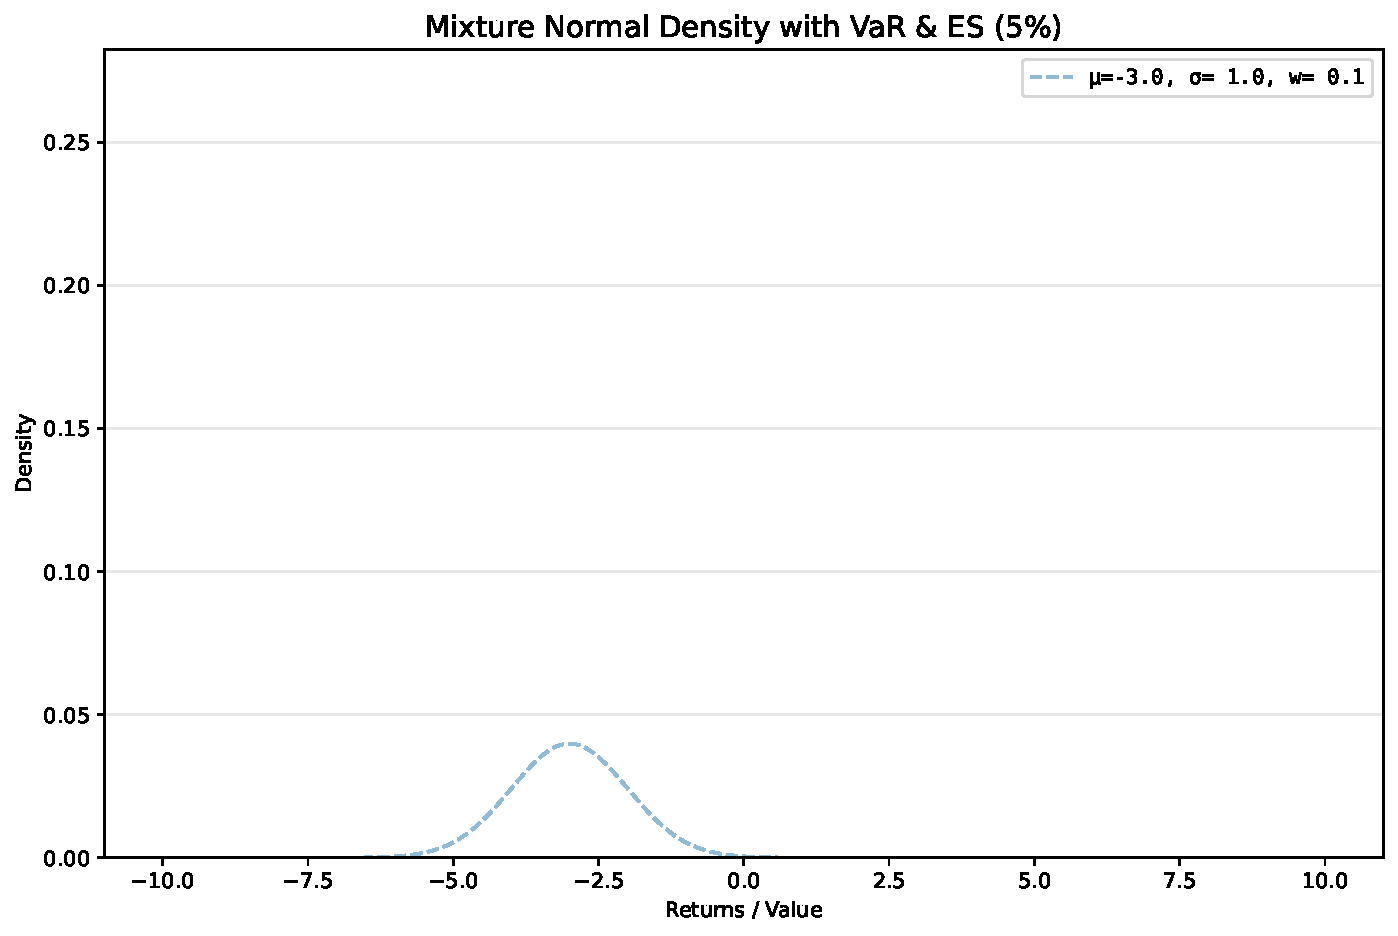
\includegraphics[width=\textwidth]{fig/slice_1_comp_1.pdf}}
    \only<2>{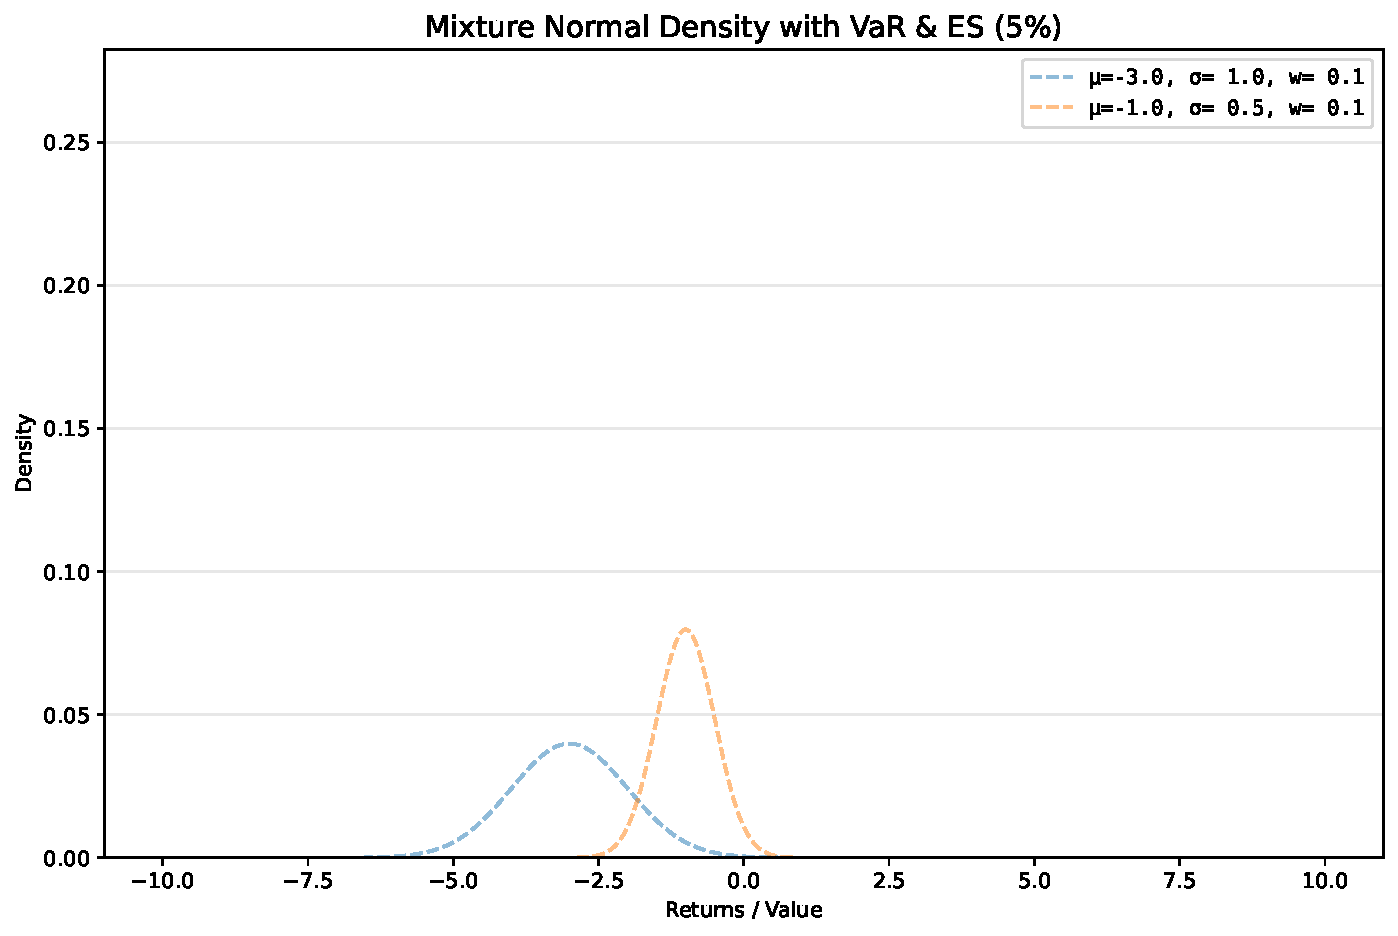
\includegraphics[width=\textwidth]{fig/slice_1_comp_2.pdf}}
    \only<3>{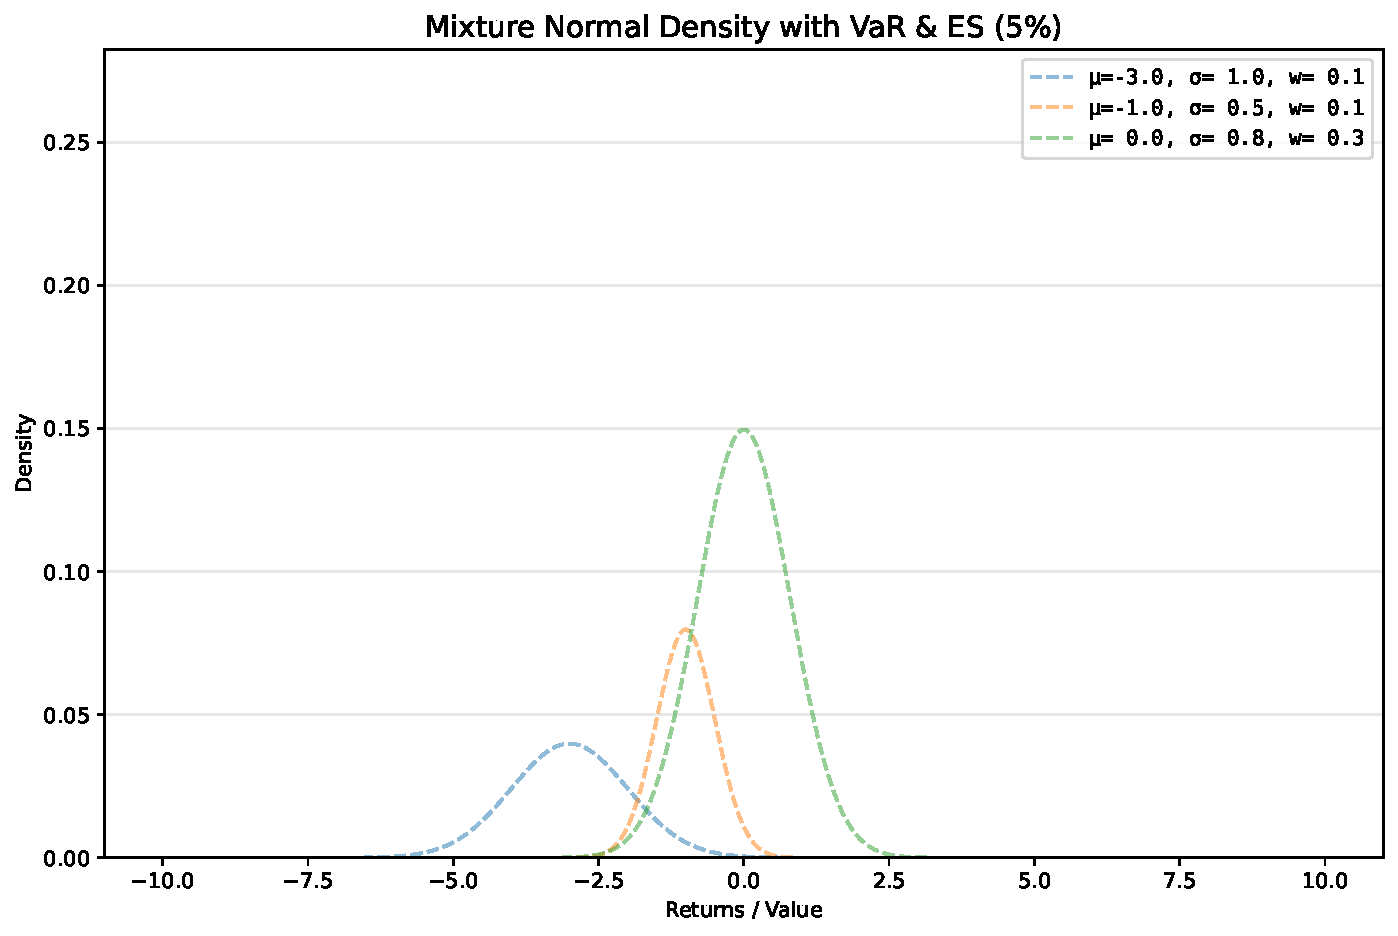
\includegraphics[width=\textwidth]{fig/slice_1_comp_3.pdf}}
    \only<4>{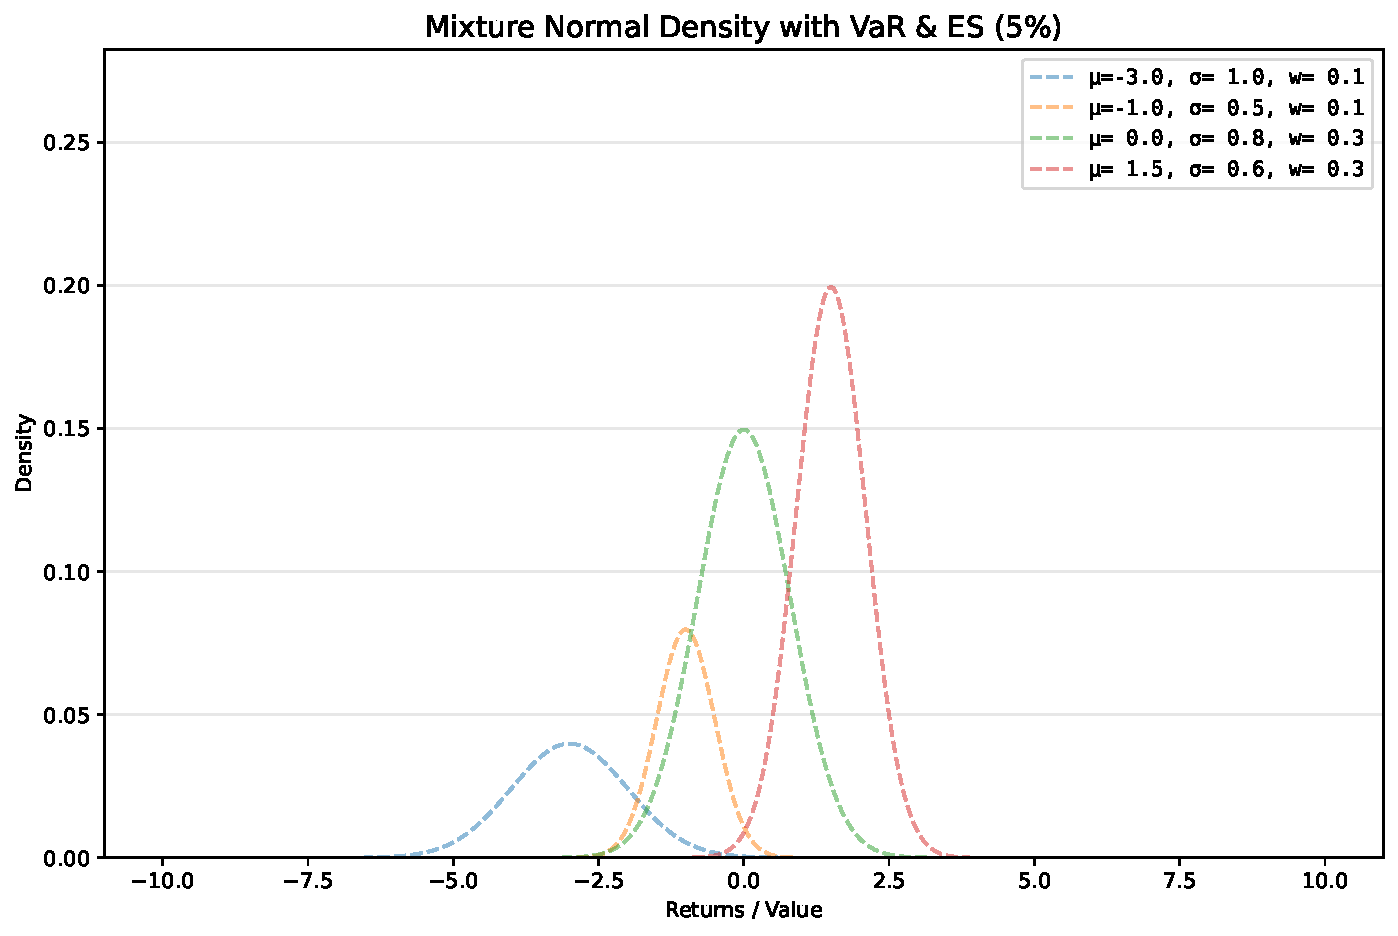
\includegraphics[width=\textwidth]{fig/slice_1_comp_4.pdf}}
    \only<5>{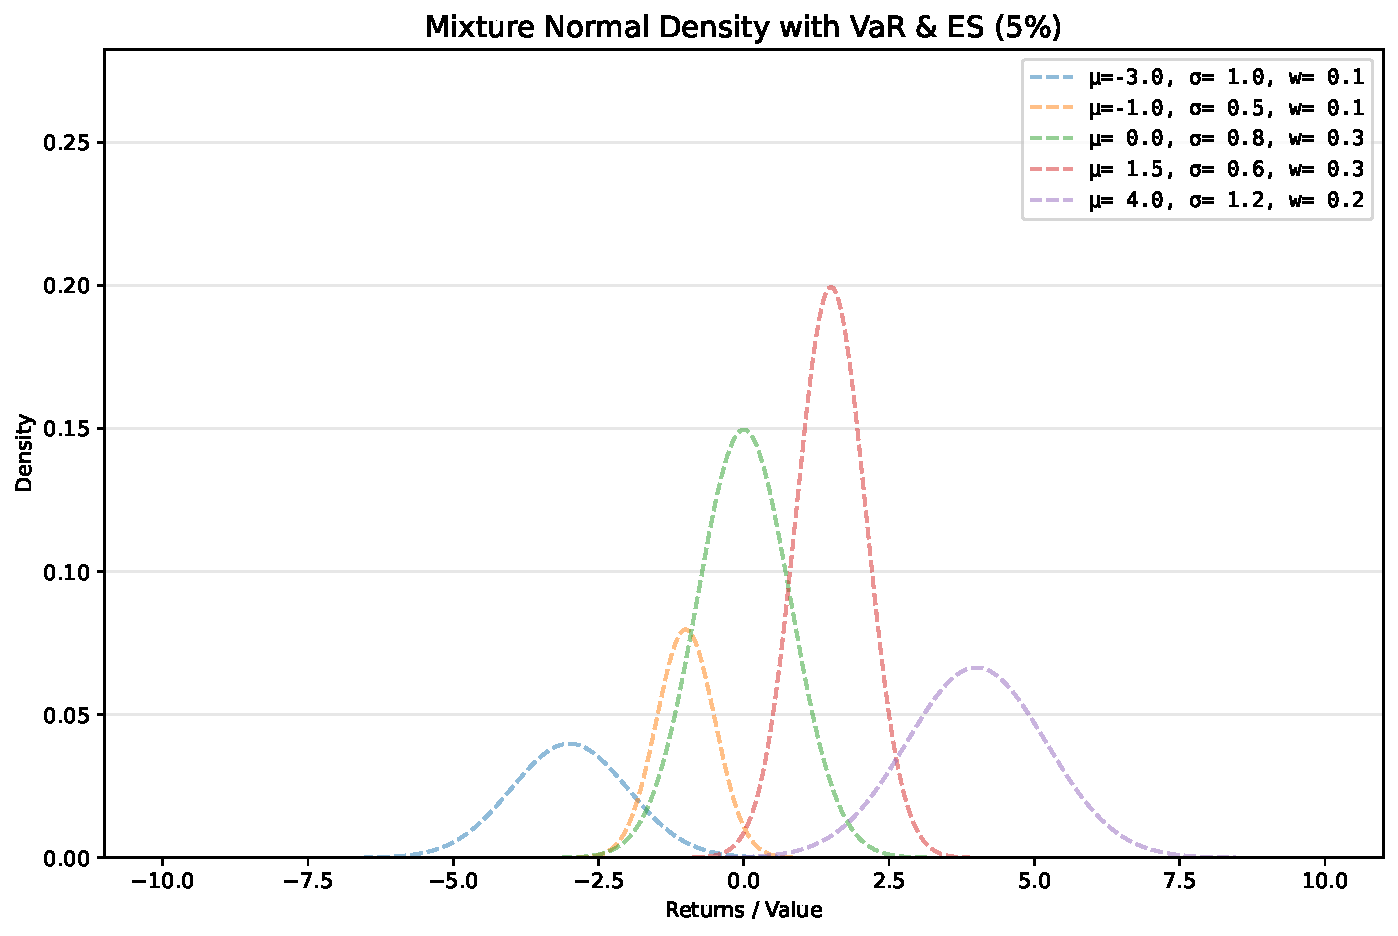
\includegraphics[width=\textwidth]{fig/slice_1_comp_5.pdf}}
    
    % --- 第二阶段：黑色的 Mixture 混合线浮现 ---
    \only<6>{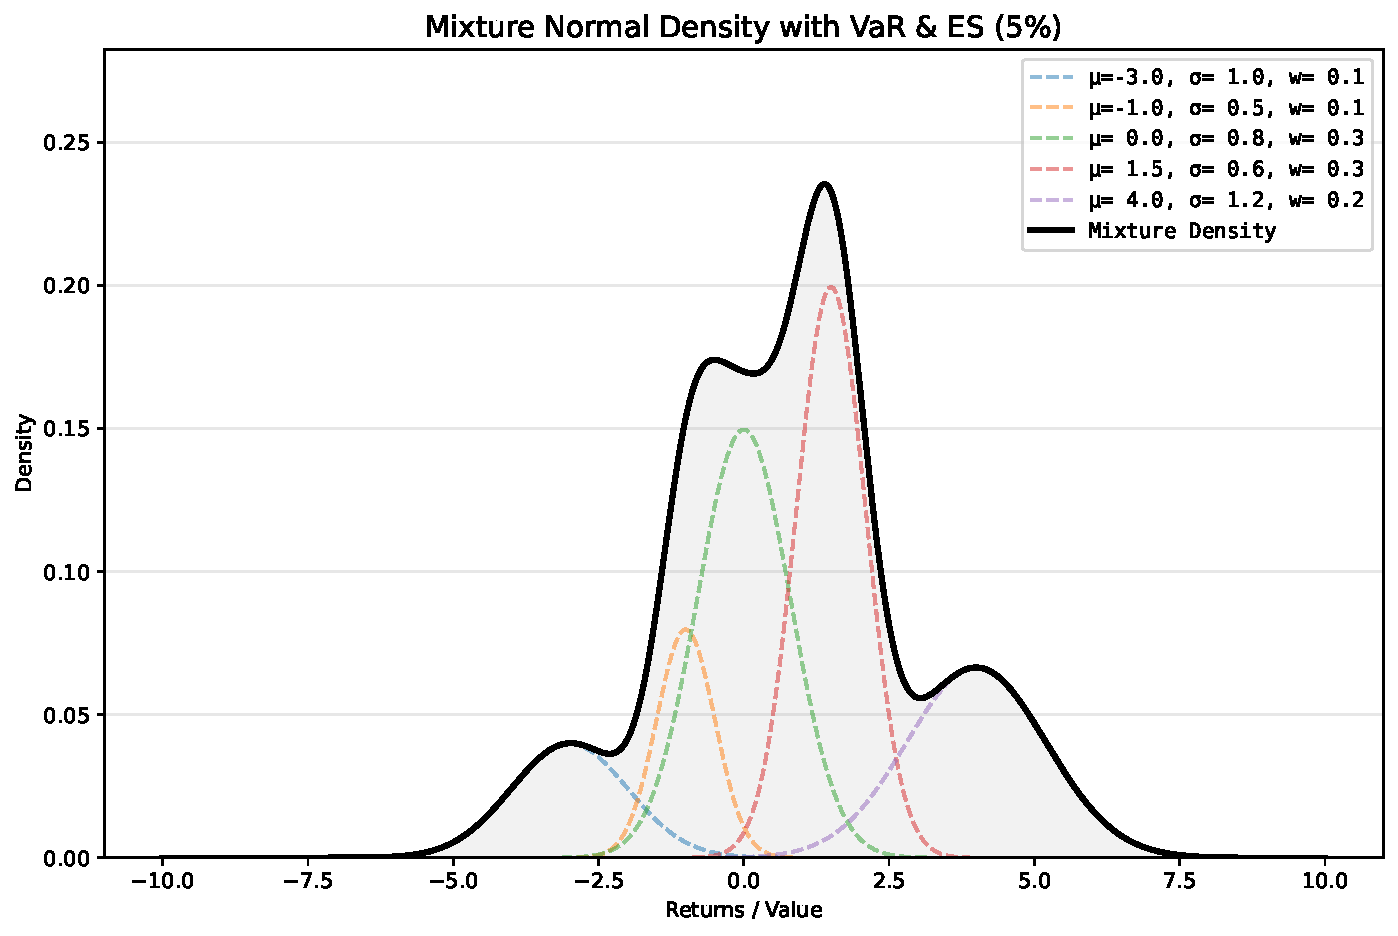
\includegraphics[width=\textwidth]{fig/slice_2_mixture.pdf}}
    
    % --- 第三阶段：红色的 VaR 尾部风险区域浮现 ---
    \only<7>{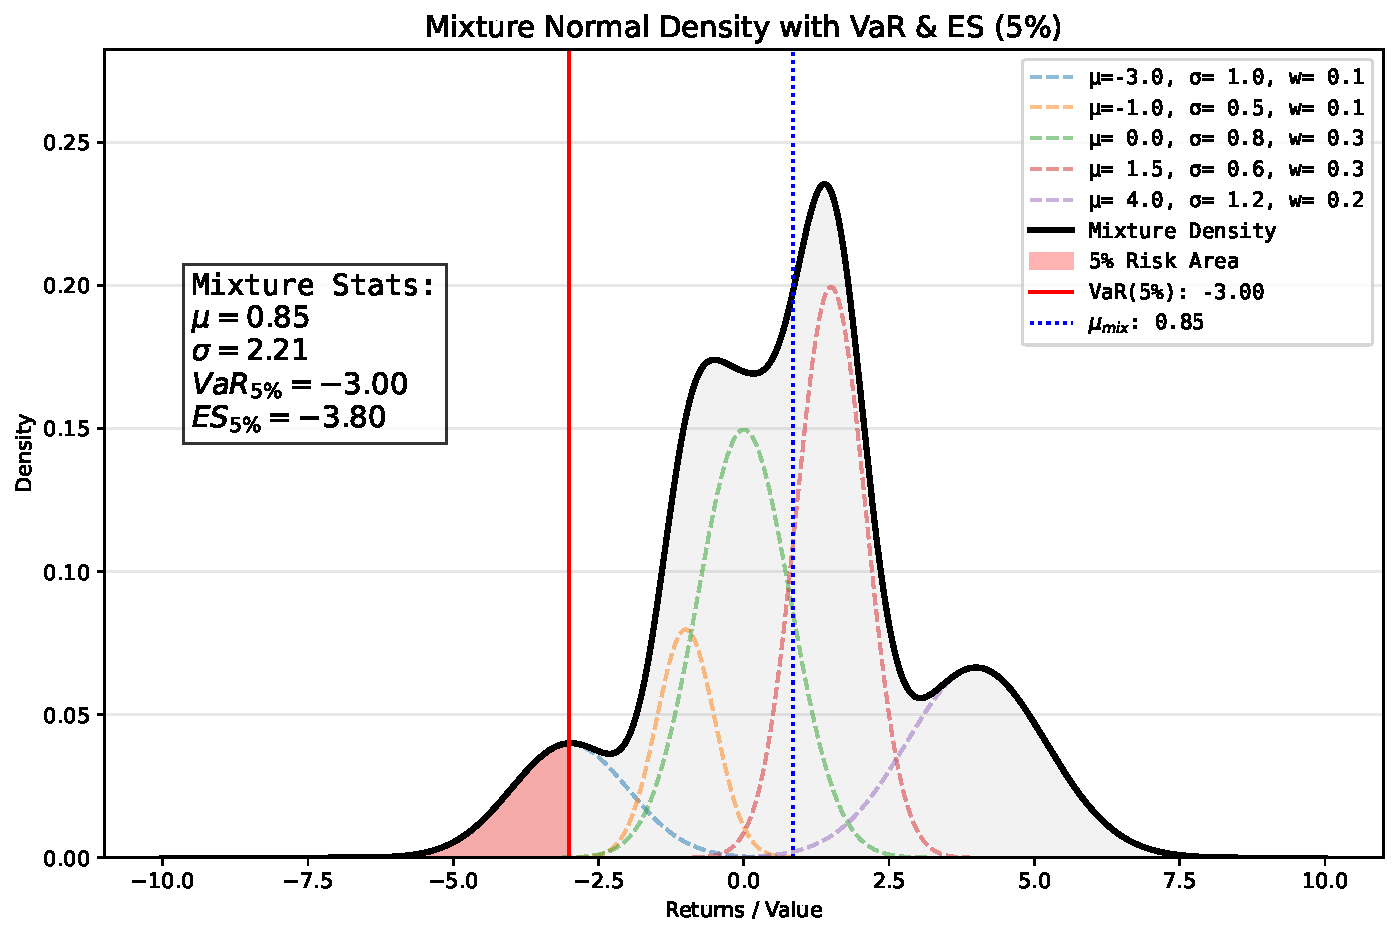
\includegraphics[width=\textwidth]{fig/slice_3_final_var.pdf}}
\end{frame}

\end{document}